\documentclass{article}
\usepackage[english]{babel}
\usepackage{csquotes}
\usepackage{amsmath}
\usepackage{url}
\usepackage{comment}
\usepackage[a4paper, total={6in, 8in}]{geometry}
\usepackage{gensymb}
\usepackage{graphicx}
\usepackage{subcaption}
\captionsetup[subfigure]{font={bf,small}, skip=1pt, margin=-0.25cm, singlelinecheck=false}
\captionsetup[figure]{font = {small, stretch = 1}}
\usepackage{chngcntr}
\counterwithin{figure}{section}
\counterwithin{table}{section}
\usepackage{tabularray}
\usepackage{xcolor}
\graphicspath{{./Figures/}}
\usepackage{float}

\usepackage[
backend=bibtex,
style=authoryear,
sorting = ynt
]{biblatex}
\addbibresource{Thesis.bib}

\renewcommand{\baselinestretch}{1.5} 

\title{My masters}
\author{Simen Storesund}
\date{\today}


\begin{document}
    \maketitle
    \section{Introduction}
    \subsection{Animal Navigation}
    One baffling observation from the study of animal biology and neuroscience is how easily animals are able to grossly outperform human-made robots. This is true over a wide scale: not only are birds able to repeatedly and consistently trek thousands of miles between two locations each year, but a range of animal studies show how for instance mice flexibly and reliable learn to adapt to their novel environments, seemingly using a broad range of environmental cues, as well as self-motion.
    In 1948, Edward Tolman connected observations of navigating rats to a term he coined a cognitive map \parencite{Tolman1948}. This was too early to have any suggestion for the neural basis of a cognitive map, and instead based on how rodents solved certain maze problems.

    For instance, in one task described in a 1946 paper, a rat would enter a circular hub from a south arm \parencite{Tolman1946}. From the hub, the only other exit was to the north. This exit led to winding corridors and eventually a reward in a location that was ultimately north-east of the starting circular area.
    After conditioning on this northern pathway and the reward, the rat would enter the circular area to find that the northern path was blocked - instead, a series of radial arms had appeared at different outbounding directions from the hub. Rats, put in this central hub, seemed to prefer radial arms of approximately north-eastern direction, which indicated that what they learnt, during conditioning, wasn't just a stimulus-response reaction, in which they learnt to run straight forward upon entering the hub, do the exact turns needed, and get the reward. Instead, Tolman argued, the rat learned some kind of map of the environment, leading to knowledge of where the reward-location was, relative to the central hub. The more comprehensive this map would be, the more flexibly the rat would be able to navigate the world.

    Since then, spatial navigation and cognitive maps has been extensively studied both on a behavioral and a neuronal level, leading to a wealth of observations on how the brain does what human-made robots cannot \parencite{Dudchenko2010}. However, since Tolman, some debates have been running as to the extent of this cognitive map, and what drives it. One central topic is whether the cognitive map is formed by path integration or external landmarks, or which one is preferred. Path integration is thought to use proprioceptive and vestibular information to estimate the animal's velocity during movement, which can be integrated in time to form a cognitive map. The benefit of path integration is that it doesn't rely on external senses, and is as such extremely flexible in a series of conditions, but it struggles due to accumulation of noise over time. 
    Remarkably, removing a hamster from their nest in pitch darkness and placing them in the middle of a surrounding open field reveals that they will return directly to their nest. Meanwhile, if the underlying environment is carefully rotated,the hamster's showed a slight tendency to go in the direction their nest would have been before rotation \parencite{Etienne1980}. Further papers show rodents', and other animals', ability to home, or find a straight path from some location to a home location, following spatial exploration. However, pure integration, without any external cues, is only seen to work over short distances in both rodents and humans.

    Navigating with external landmarks is also extensively tested. A typical example is the radial arm maze, in which a rodent is placed in the center of a room with a number of radial arms, typically eight, in which each might be baited with food. Rodents are typically able to extract food by visiting each arm only once, showing some kind of memory of where they have been. However, if given a series of external landmarks, that are placed on walls outside the maze, and these landmarks are either rotated or shuffled after the rodent has visited three out of eight arms, the following performance drops significantly \parencite{Suzuki1980}. The benefit of using external landmarks or sensory cues is that chosen well, they tend to be invariant in time, providing allocentric navigational information. This makes them robust to noise and drift. However, landmarks are only useful as long as these landmarks can be observed.
    
    
    \subsection{The Transition Scale Space Model}
    The transition scale space model (TSS) seeks to explore how such a mental map would look, from a computational perspective \parencite{Waniek2020}. The model goes beyond spatial navigation, but the principles it operates under can easily be extended to a spatial environment, and posits, initially, that any model-based path finding system would require two separate memories: a mental map, or some internal representation of the environment, and some way to connect locations on this map together to get sequential routes between some start and some goal.

    While the physical space as experienced by mice is a continuous two-dimensional plane, any cognitive map of the environment must be represented by discrete neurons. This discretization of space could occur in many ways, but matching experimental observations, the TSS model suggests that this map could be a network of neurons in which each represents single locations in an environment. Part of the purpose of this network is storing information about each location, which is central for navigation: during path-planning, a mouse must be able to selectively avoid locations that are considered dangerous, which can be based on experience of those locations. The cell in this map-network representing 'home' would elicit very different responses from the cell representing a dangerous territory, for instance if the mouse has encountered predators there previously.

    Such a network does not necessarily contain information about how locations are connected, spatially. Each node, or cell, in the network, does not know its own neighbors. This information is necessary for spatial navigation, and the TSS-model posits that this information can be stored in another network. In this network, each cell represents spatial transitions, to give information about which locations are available at a certain distance from a current location. However, due to the considerable number of possible spatial transitions, making each cell represent a single transition would require a high number of transitions, so the TSS model instead suggests letting each transition cell represent multiple transitions.

    The one constraint is that the network breaks down as soon as a transition cell represents a transition both to and from the same location - the domain of the transition cell, which are the places the transition cell transitions from, and the image, where it transitions to, must be disjunct. Apart from that, each transition cell should represent as many transitions as possible, to minimize the number of cells necessary in a working transition cell network.

    This argument stands at the center of the TSS model, because it posits that if a mouse brain indeed has these transition cells, they would be as efficient as they could be, appealing to the second level in Marr's three levels of analysis - in a biological network, any cell with a particular purpose should behave as to fulfill that purpose optimally, whatever the purpose is.
    Through mathematical derivations, the TSS shows that such a transition cell operating under the constraints listed above would have a striking spatial activity pattern. Although the mathematics won't be reproduced here, the logic behind an optimal transition cell is as following:
    a transition cell will be activated by all place cells in some limited region, referred to as a 'center' region, and will represent all transitions from that center to all place cells in a region surrounding this center, the 'surround' region. The transition cell will try to fit as many of these 'center-surround' regions into the environment as possible, as long as there is no overlap between center-areas and surround-areas.

    Indeed, in the limit of getting as many center-regions into the environment as possible, this transition cell will be active in a periodic, hexagonal pattern in an open environment, which is a solution derived from the sphere-packing problem in two dimensions \parencite{Waniek2018} [Cite sphere packing here?]. With optimal transition cells, all possible spatial transitions from center-areas to surrounding areas can be encoded in a network of only three such cells, highlighting how effectively these cells represent spatial transitions.

    A variable in these transition cells is the size of the center- and surround-areas, which in turn would influence the scale of the hexagonal activity pattern. A transition network as described in the TSS-model would work best with multiple separate scales, so larger scales can accelerate the retrieval of paths. In biological systems, where a transition cell has a rate coded activity in a gaussian for each center region, the ideal increment between scales is the \(\sqrt{2}\).

    On this basis, the TSS model predicts two memory structures in animals:  internal map, which consists of neurons representing single locations, and a network of transition cells trying to bundle as many transitions together without spurious transitions. Cells in the internal map-network should activate preferentially when the mouse is in some signature location, and cells in the transition-network should show a hexagonal firing pattern, representing available spatial transitions. This transition-network should also contain transition neurons on different scales, in which the increment from one scale to the next is the \(\sqrt{2}\).
    
    \subsection{Spatial Cell Types in the Hippocampal Area}
    The following section will describe experimental results supporting and opposing these predictions made by the TSS model.
    Already fifty years ago, the place cell was observed in the mouse hippocampus, and this has led to a series of interesting experiments and observations \parencite{OKeefe1971,OKeefe1976}. Interestingly, the hippocampus was of interest because of its importance in episodic memory formation. The canonical hippocampal pathways divide the hippocampus in three regions that communicate in a feedforward manner: the dentate gyrus receives inputs from outside the hippocampus, and project these to CA3, which both has recurrent excitatory connections as well as projections to CA1 [Source here?]. The main output region from CA1 is the subiculum, which is outside the hippocampus and projects to the prefrontal cortex. Place cells have both been observed in CA3 and CA1, but have not been seen outside the hippocampus.

    The place cell typically fires with a rate that is distributed in a gaussian around one or a few locations in the environment, so a network of place cells can encode all positions in an environment \parencite{Wilson1993}.
    One line of evidence that suggests that place cells participate in navigation is sequential activity, observed both during and after navigation. Sequential place cell activity during rest or sleep after navigation, called replay, reflects both sequences of place cells in the order they were active during navigation, or reverse sequences \parencite{Wilson1994}. Interestingly, replay occurs during sharp wave ripples, in which the place cell activity is temporally compressed relative to their activity during navigation.

    Preplay refers to sequential place cell activity during navigation. During preplay, place cells corresponding to the current location is followed by place cells that will be active a short time into the future, indicating that the hippocampus has some information about upcoming place cells \parencite{Dragoi2011,Dragoi2013}.

    The hippocampus is also subject to oscillations in the local field potential, prominently in the 4-11 Hz region, called theta oscillations, or just theta. When preplay is viewed relative to theta, the place cells corresponding to the current locations are active at the trough of the wave, while past place cells activate in the descending part of the wave, and future place cells activate in the ascending part of the wave. This phenomenon is called theta phase precession \parencite{OKeefe1993, Skaggs1996,Hafting2008}.

    Replay typically occurs during rest or sleep following explorations, in which sequences of place cells experienced prior to rest are activated again, but compressed temporally (Tonagawa)\parencite{Olafsdottir2016} . Moreover, combinations of sequences are seen, which seems to produce novel trajectories in an already explored space.

    Interestingly, place cells can be active in multiple environments, but they remap independently of each other \parencite{Muller1987}. This implies that the place cell networks are modulated by the context, but the mechanisms for this are currently unknown.

    Grid cells were originally found in the search of afferents to the hippocampus place cell system, first found in layer II of the medial entorhinal cortex (mECII)\parencite{Hafting2005}. Grid cells are characterized by periodic spatial activity, arranged so that the firing fields make up hexagonal patterns spanning the environment, and this activity is found both in stellate- and pyramidal cells of mECII\parencite{Rowland2018}. These cells are also firing independently of head direction or velocity, and have since been found in multiple other parts of the brain, such as in deeper layers of the medial entorhinal cortex (III - IV), as well as the pre- and para-subculum (Cite these here).

    Grid cells, too, have received a lot of attention, and a series of details about their firing properties has since been revealed. Grid cells seem to align with the boundaries of their environment with a small wall-angle offset, and grid cells located near each other in the entorhinal cortex also share the spacing, or size of each hexagon (Some other sources here?). However, along the dorsoventral axis, the spacing of the grid increases by a factor of the square root of two (Also, source?). Grid cell activity is strikingly robust across trials and time, and it also seems to persist when visual cues are removed (Source). However, their hexagonal gridness depends on the environment shape, and their firing pattern gets distorted in trapezoid or not-regular environments \parencite{Stensola2015,Krupic2015}.

    Grid cells also exhibit theta phase precession during navigation \parencite{Hafting2008}, and interestingly, when abolishing the theta rhythm by lesioning the medial septum, grid cell activity loses their spatial correlation in mice, so theta rhythm seems critical for the grid cell pattern \parencite{Brandon2011,Koenig2011}. However, this was not seen in similar experiments in bats \parencite{Yartsev2011}.

    Typical input regions to the medial entorhinal cortex are the post- and perirhinal cortices, as well as the pre- and parasubiculum, which seem to integrate information from multiple sensory modalities, but to the author's knowledge, the concrete input structure to grid cells is not known (Multiple sources required here, lol).

    Within mECII; grid cells seem to be interconnected by parvalbumin-positive interneurons, applying strong, lateral somatic inhibition, while excitatory connections have not been observed \parencite{Couey2013,Buetfering2014}. Moreover, maturation of this interneuron structure seems to reinforce and strengthen the spatial correlations of grid cells \parencite{Christensen2021}. 
    Connectivity between grid cells and place cells are only partially mapped, but in addition to the canonical tripartite synapse model, which understood the dentate gyrus as the main input region of the hippocampus, the mECII also projects directly to CA1 (Check Witter’s review, find sources there). This suggests that place cells might be formed based on summation of grid cell inputs on multiple scales, but this idea was contradicted when it was found that place cells mature earlier than grid cells in development (postnatal day 16-17 versus postnatal day 19-20) \parencite{Langston2010,Wills2010,Wills2012}. However, it has been established that CA1 also projects strongly back to mECII, and that grid cell activity depends on these connections \parencite{Bonnevie2013}.

    \subsection{Existing Grid Cell Models}
    A multitude of models and model families already exist to explain the wealth of experimental data on grid cells, with differences in their suggested mechanisms for the grid pattern, as well as the purpose of the grid cell. Due to their persistent spiking in darkness, many models assume that grid cells do path integration, integrating self-movement information to predict current location in the absence of external inputs(Hafting, plus a bunch of models, or a review?). Oscillatory interference (OI) - models seek to explain the theta phase precession in grid cells, and have shown that grid-like activity can be achieved by the interference of multiple oscillators in membrane potential \parencite{Burgess2007,Zilli2010}. The OI-model can account for many activity patterns, but if the different oscillators differ in frequency by a sufficiently small margin, and adapt this margin based on speed- or velocity-signals, the cell can have a grid-cell-like activity with spacings as observed in experiments. Also, these methods effectively explain the phase precession observed in grid cells. 

    Another set of models explain the grid cell as a part of a continuous attractor network (CAN), which can explain persistent grid cell activity during rest or sleep \parencite{Yoon2013,Widloski2014}. These models can be implemented with lateral inhibition between grid cells, as observed in mECII, as long as the strength of the inhibition is inversely proportional to the overlap of firing fields, so the most active grid cell silences all other grid cells. When the animal moves, this activity is shifted to a grid cell with a neighboring phase.

    It has been demonstrated that any such system of path integration still needs regular external input to avoid drift, and the exact inhibitory structure predicted by CAN - networks have not been observed. Additionally, the velocity-based inputs have not been observed, although this might just stem from the unexplored input-space of grid cells (Some review claimed this).

    A third group of models predict that grid-patterns can be learnt by Hebbian learning, which is by associating to the right spatial inputs and dissociating from other spatial inputs. As opposed to the OI- and CAN-models, the driving mechanism of grid cell activity in these feed-forward models is not necessarily self-motion inputs, put that doesn't necessarily exclude the possibility that grid cells participate in path-integration. 
    
    An early idea was to model this using firing fatigue, in which grid cells received inputs from cells with rate-based place cell-like activity, although they were not claimed to actually be hippocampal place cells \parencite{Kropff2008}. In this model, there were two primary factors for learning - competitive firing rates between grid cells, so the total population rates were normalized, as well as a firing fatigue, so prolonged firing would reduce rates. Grid cells would then associate to place cell inputs based on their mutual rates, and the fatigue prevented the same grid cell from associaing to all inputs. While this produced grid-like cells, carefully tuned excitatory collaterals between gridcells were necessary to make them share orientation.
    Later, this excitatory collateral was replaced by inputs from a layer of collateral cells that received both place cell-input and head direction-cell input, so the model produced grid cells with shared orientation in a purely self-organized manner \parencite{Si2013}.

    Some models produce grid cells with a center-surround learning rule from place-cell inputs. In these models, grid cells typically associate to place cell inputs with firing fields with a given distance, and dissociate from place cells with firing fields outside this distance. Mercade and Leibold showed that this learning rule, combined with lateral inhibition, reduced boundary-effects on grid formation and showed a high level of gridness \parencite{Mercado2020}. While the grid cells prefered an orientation around 7.5 degrees, in line with experimental results, but all grid cells were found in one of three distinct phases. Another feedforward model added a second ring around the center-surround area, and place cells within this narrow ring were tagged so new firing fields can only occur on the narrow ring. Moreover, if a place cell gets tagged from two separate firing fields of one grid cell, the weights would potentiate. While this was robust to noise, it is unclear if orientations and phases would align between grid cell \parencite{Castro2014}.

    The observation that center-surround plasticity can lead to gridness is reminiscent of ideas from the TSS model. In the TSS model, the suggested mechanism by which transition cells learn is suggested to be similar to how place cells learn their receptive fields. The place cell learns to activate based on spatially modulated sensory inputs, in which each place cell associates to spatial inputs from one area, and lateral inhibition prevents other place cells from activating. This has been explored in numerous works prior to TSS, for instance using boundary vector cells or object vector cells as inputs \parencite{Barry2006}(am I correct saying this also exists for OBCs?). Boundary vector cells and object vector cells are similar in that they activate preferentially when the animal is at some distance and direction relative to an external structure. Cells are called boundary vector cells if this structure is an environment boundary, such as a wall or a cliff, while they are called object vector cells if the structure is some environment landmark. Using cells like these as spatial input in a feed-forward network is attractive because the cells can plausibly exist and be configured prior to exploration, and computed during exploration through optic flow \parencite{Raudies2012}.

    \subsection{Grid Cells as Potential Transition Neurons}
    Under the TSS-model, grid cells, which are suggested transition cells, are also formed from spatially modulated inputs. As opposed to place cells, these associate to spatial inputs in center-regions, and dissociate to inputs from the surrounding-regions, while trying to fit as many center-regions into the environment as possible. These transition cells are also interconnected by strong lateral inhibition, to discourage overlapping center-regions.
    Notably, the TSS-model only assumes this learning rule for the lowest transition-scale, while subsequent scales can be learnt recursively from inputs on the last scale.

    This learning rule has been proven in discrete-time simulations in networks of three transition cells, which received spatial inputs sampled from a regular, rectangular grid of spatial cells. In discrete time-steps, activity in the spatial cell layer would activate transition cells depending on a position in a simulated trajectory. Following this, three separate learning rules would update input-to-transition cell weights. The first rule would let the most active transition cell associate to the nearby spatial cells, and dissociate from surronding spatial cells. The second rule, called the baseline, would increase the weights from the active input cells to all transition cells, regardless of their activity. Third, an interaction rule would weaken the connection from inputs to all transition cells except the most active one.
    A rationale for the three learning rules is that the first rule provides the center-surround effect necessary for transitions, the baseline encourages transition cells to be active as frequently as possible to encourage effective transition cells, and the interaction rule discourages excessive overlap between transition areas.
    
    Although this network gave cells with high gridness in networks of three transition cells, demonstrating that the TSS-model can give rise to transition cells, it did not work in bigger networks. This is necessary in a biological network. Additionally, it is unlikely that a biological network providing the spatial inputs shows regularly distributed, place like activity. Both of these constraints need to be addressed for this network to be considered biologically plausible.
    In this work, the main objective is to build upon these simulations, and establish this network structure in a more biologically plausible way, and explore under what conditions or constraints transition cells develop a hexagonal structure. 
    This task is divided in two. First, to see if a biologically plausible network can contain more than three grid cells, by simulating in continuous time with delayed inhibition, so the grid-dissociation is partial instead of complete.
    Second, the way the structure of spatial input affects gridness is also explored. To allow for a center-surround learning rule, spatial input was always phase-coded, so the grid cells received pulses of inputs in simulated theta-cycles, in which the more relevant inputs arrived earlier, and a STDP-learning rule separated center from surround input. For highest biological plausibility, this input would be boundary vector cells or similar, and this was attempted with complex dendritic computations to allow differentiating vector-inputs, but place-cell like distributions were also attempted to reduce the simulation complexity and simulation times. With a simple STDP- based learning rule, robust gridness scores were observed with multiple network structures, showing that cells can learn spatial transitions effectively under biologically plausible conditions.
        
    \section{Methods} 
    \subsection{Overall model design and -goals}
    The purpose of this thesis is to test gridness in transition neurons as described by the TSS-model with biologically plausible spatial inputs and conditions (continuous time). To achieve this, transition cells were simulated in a spiking neural network, which are artificial networks with certain properties:
    \begin{enumerate}
        \item The network is simulated with continuous time, or in time steps that are significantly shorter than the mean firing rate of neurons.
        \item Neurons communicate in temporally discrete spikes, triggered when an internal voltage variable exceeds a threshold.
    \end{enumerate}
    
    Different network structures have been tested over the course of the thesis, and the results of different structures are treated in the results section. This section will first describe an ideal network, and describe the different assumptions that network would operate under. The further sections will describe other network structures that were used to simplify and test different levels of plausibility.

    An ideal network has the following properties: it is simulated in a biologically plausible network, such as a spiking neural network. Most importantly, this means that communication happens at a delay, time is continuous, and learning rules must be online and local. Simulations get inputs from some plausible spatially tuned neurons, more precisely boundary vector cells (BVCs), whose activity is based on real or simulated trajectory data. From these inputs, another layer of cells of arbitrary size learns center- and surrounding area information to represent transition-cells as described in the TSS-model, encoding transitions on a single scale. Under these constraints, the objective is whether the transition neurons self-organize into single-cells with hexagonal activity patterns in space, and in which the population covers all possible environment transitions.

    Both an ideal network and subsequent simplifications will have some common features to accommodate these limitations: first, spike timing dependent plasticity is a biologically plausible learning rule which both allows single transition cells to associate with spatial inputs associated with center, and dissociate with inputs associated with surround areas. To facilitate this, all inputs arrive in pulses at theta-wave frequency, 10 Hz, in which only spatial input with sufficient relevance is active. The input is also phase coded, so the less relevant, the higher the temporal offset is relative to theta. This means that a transition cell is likely to fire following center-inputs, and subsequently receive a burst of inputs from cells representing surrounding locations. The STDP learning-rule will ensure that the center-activity which arrived pre-spike are potentiated, and the surround-activity arriving post-spike is depressed. Secondarily, all active inputs are slightly potentiated to encourage the transition cell to be active in as many center-areas across the environment as possible.

    \begin{figure}[htbp]
        \centering
        
        \begin{minipage}[b]{0.59\textwidth}
            \centering
            \subcaption{}
            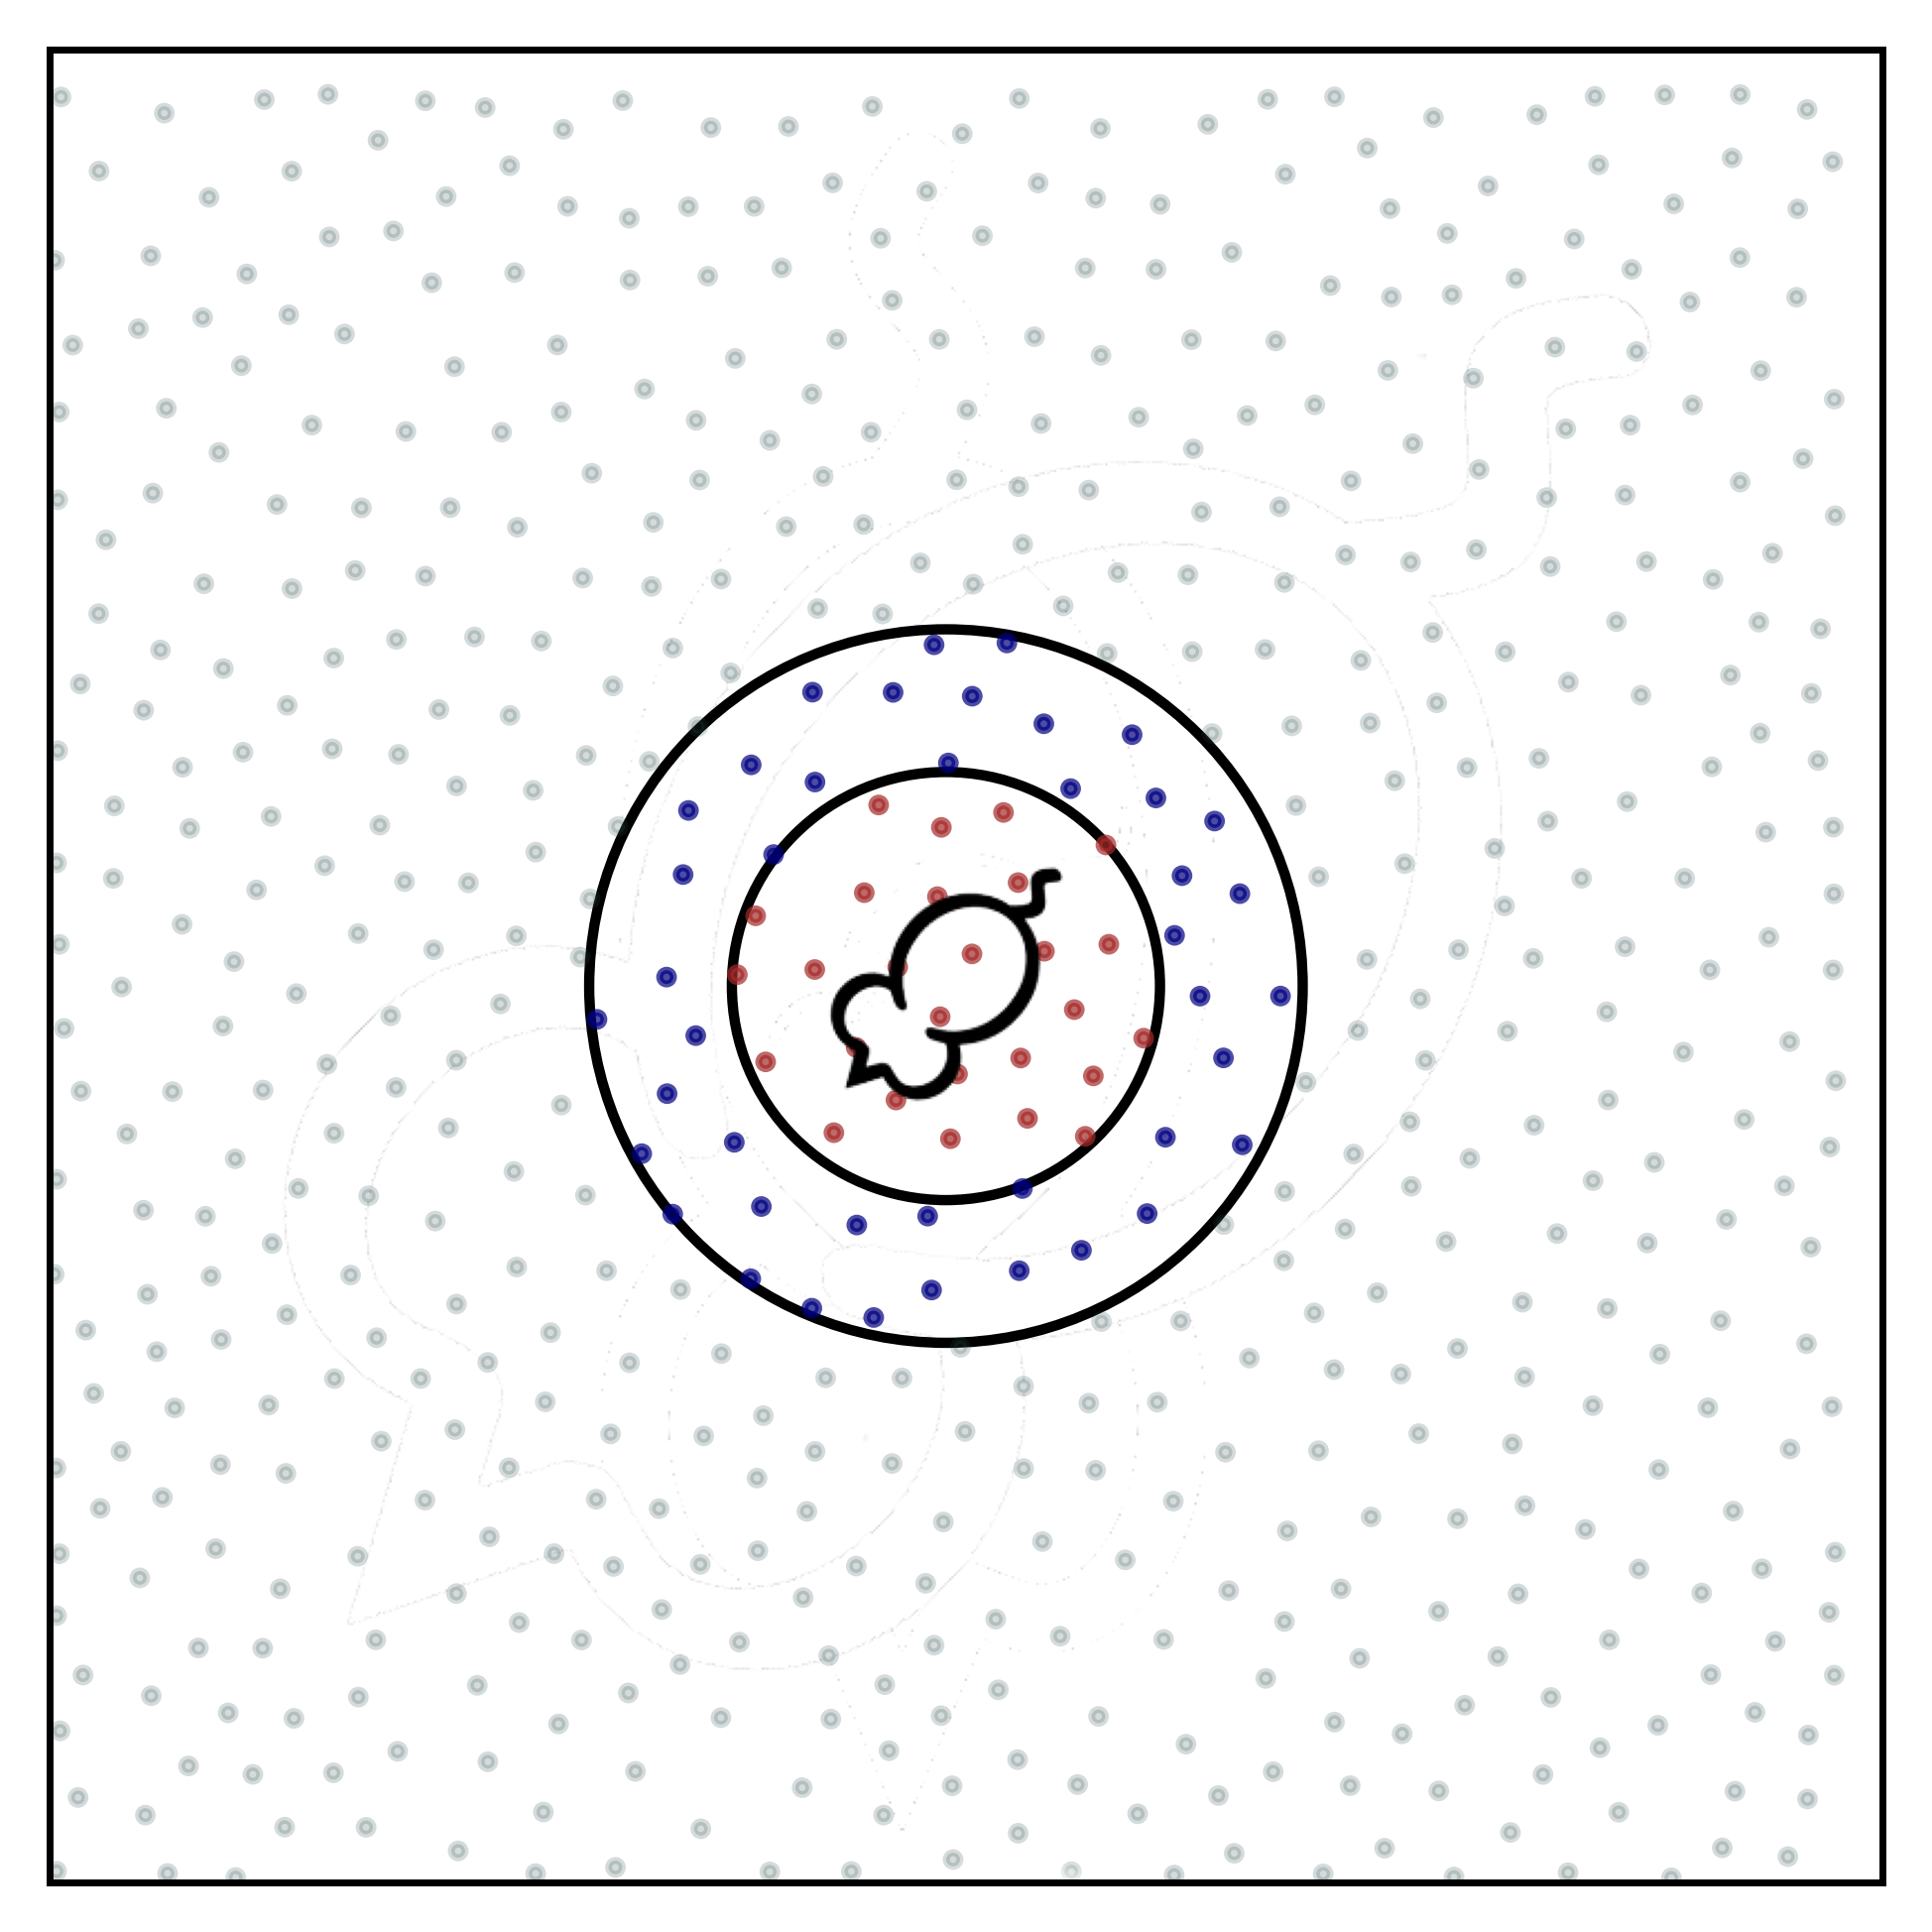
\includegraphics[width=\textwidth]{mouse_plot.png}
        \end{minipage}
        \begin{minipage}[b]{0.38\textwidth}
            \centering
            \begin{subfigure}{\textwidth}
                \subcaption{}
                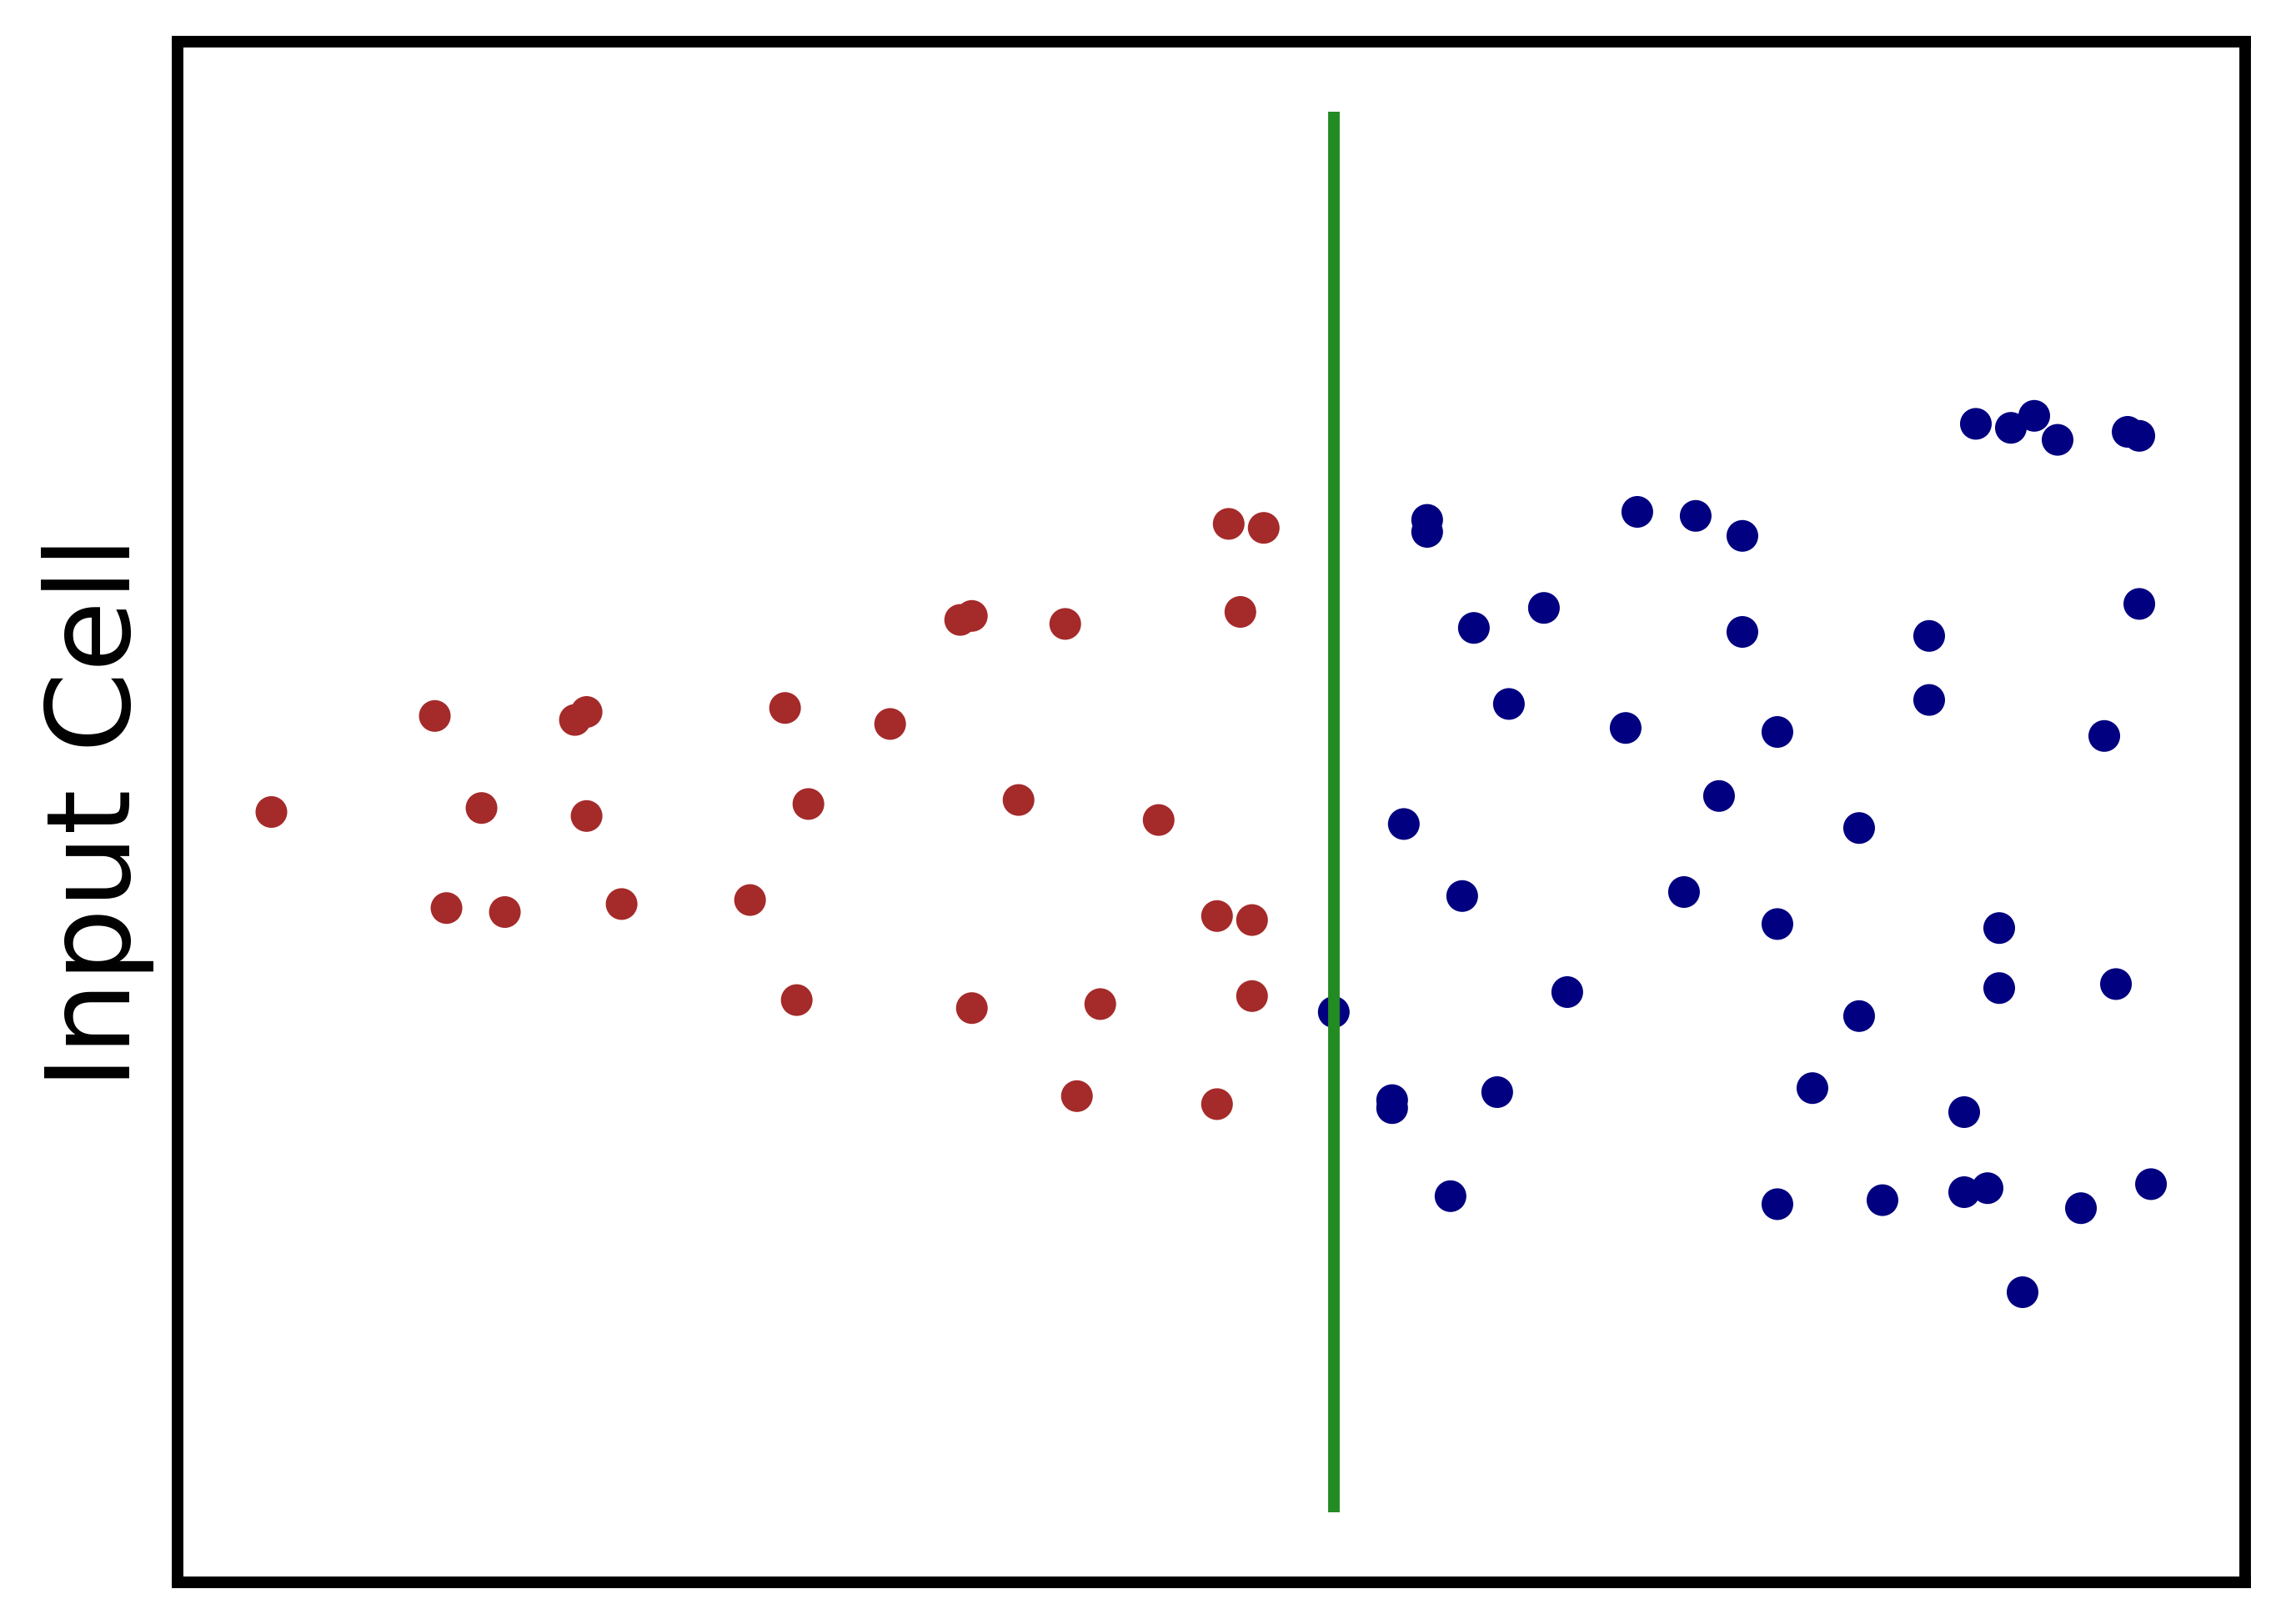
\includegraphics[width=0.95\textwidth]{input_STDP_plot.png}
            \end{subfigure}
            
            \medskip
            
            \begin{subfigure}{\textwidth}
                \subcaption{}
                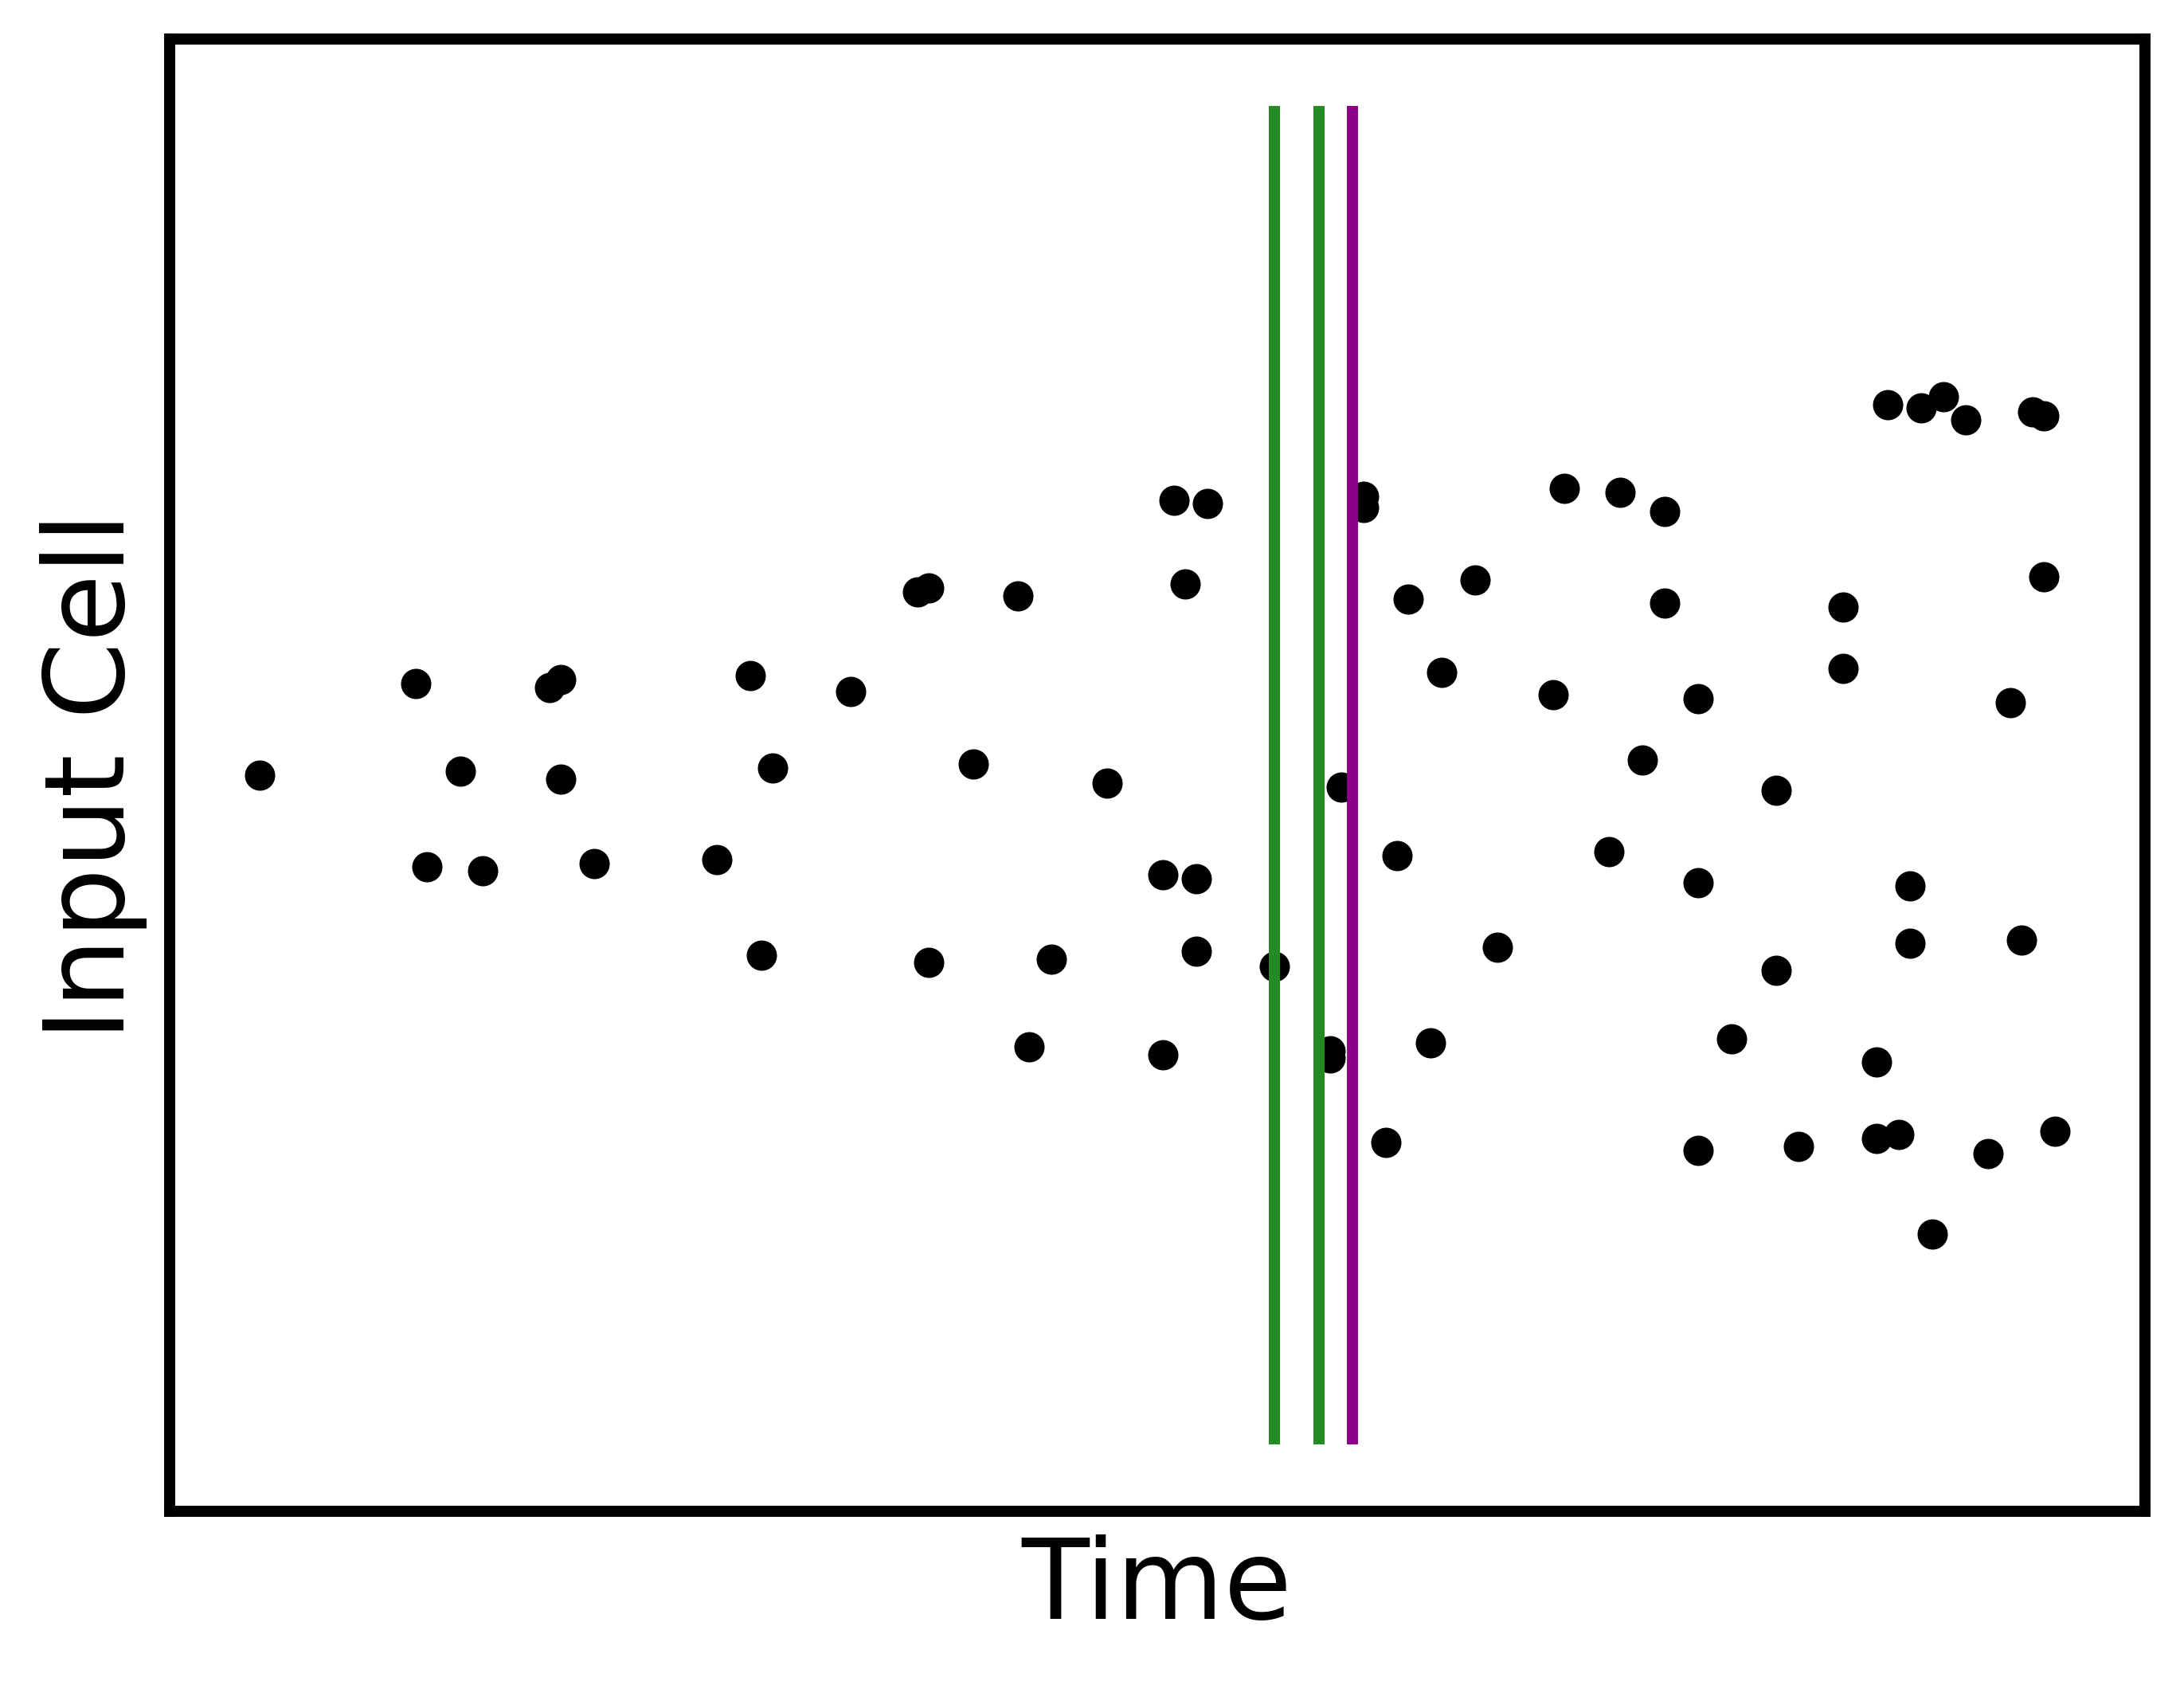
\includegraphics[width=0.95\textwidth]{input_inhibit_plot.png}
            \end{subfigure}
        \end{minipage}%
        
        \caption{(a) Spatial inputs from a region surrounding the mouse will be activated each theta-cycle, here indicated by points within the two surrounding circles. This input is phase-coded, so cells responding to locations nearest to the mouse will arrive earlier. (b) The spike time of a transition cell spike (green vertical line) is central under the STDP learning rule. The transition cell will here associate to the inputs arriving prior to spiking, and dissociate from the inputs coming after the spike. In this case, that might lead to a center- surround adaptation dynamic. (c) Delayed inhibition (purple vertical line) can allow multiple transition cells (green vertical lines) to fire during the same theta-cycle.}
        
        \label{mouse_plot}
    \end{figure}

    
    An inhibitory layer connects transition cells laterally, causing strong inhibition, but on a delay. This leaves a narrow window in which multiple transition cells can fire, followed by complete inhibition, so some transition cells partially associate to the same areas.

    Due to the high number of parameters available in such a network, the network would preferably see characteristics of the transition cells, such as grid-patterns, emerge quickly and without perfectly honing parameters.
    This is both because a network structure that produces grid cells only with very particular parameters is less biologically plausible, and because testing the parameter space properly is time consuming. On this note, there are reasons to think that a network in which grid cell activity occurs in transition cells based on linear summation of BVC input, as shown in figure 2.1, is difficult to achieve. For one, boundary vector inputs in neighboring areas are typically highly linearly correlated, so the transition cell would struggle to associate to one location and dissociate from a neighboring one. Secondly, for instance in square environments, one could imagine picking two locations that the transition cell has associated with, denoted \((x_1, y_1)\) and \((x_2, y_2)\). In locations \((x_1, y_2)\) and \((x_2, y_1)\), the input would be highly similar to half the input from position 1 and half the input from position 2, but the transition cell should not fire in these locations, because that would lead to rectangular-grid firing patterns, not hexagonal. It should be noted here that the spiking neural network itself implies non-linear features that might have enabled such a network to produce grid-cells. One way to achieve this would be with other transition cells that are sufficiently active in location \((x_1, y_2)\) and \((x_2, y_1)\), so they inhibit the first transition cell. However, due to the fine-tuning such a network would require, this network structure was not pursued further.

    An appealing alternative, which highlights the advantage of biological neurons, was to consider nonlinear dendritic computation on transition cells in a multi compartment model. Under this idea, although boundary vector cells technically synapse onto transition cells directly, the simulation treats dendrites as separate units within one transition cell. Each dendrite would get inputs from some subset of BVCs, and the transition cell can associate and dissociate to all inputs on an entire dendrite. Similarly to the BVC-model, each dendrite would preferably be active in only single locations in the environment, for instance by responding non-linearly to inputs with a soft-max activation function (as in the other paper). In the example above, this would let the transition cell associate to dendrites responding highly to \((x_1, y_1)\) or \((x_2, y_2)\), while remaining dissociated from dendrites activated in \((x_1, y_2)\) or \((x_2, y_1)\), without sacrificing biological plausibility. This multi compartment model satisfies all requirements stated above. 

    However, to shorten simulation time and reduce complexity, this kind of network can be simplified. This can be done incrementally, in which each step simplifies complexity but also reduces plausibility:
    \begin{enumerate}
        \item The BVC-model showed that place-like activity can be produced from BVC-inputs. As such, BVC-input can be replaced by place-like inputs directly as non-spiking dendrites in the multi-compartment model. 
        \item To reduce the number of neurons, each dendrite can connect to each grid-cell, and the dendrites can be spiking to reduce computational time for each of them. Here, the dendrites still fire in random places, according to some distribution.
        \item The dendrites can respond to places distributed in a regular, rectangular grid.
    \end{enumerate}
 
    Note that step 3 is highly similar to the already existing simulations by Waniek (citation?), just here in a spiking neural network. This was useful, because it allowed testing the hypothesis that transition cells can produce grid-like behavior in networks of more than three neurons if the inhibition is delayed, not showed in previous simulations. Then, networks could gradually be made more complex and biologically plausible, leading to a series of networks that could be tested sequentially from simple and less plausible to more complex and more plausible. The concrete implementation of each network and other considerations are treated in their own upcoming subsections.

    \subsection{Simulation software} All models and implementations can be found on github(Insert link here?), and while the simulation data is not available on github due to storage capacity, it is available (somewhere else?). All simulations were implemented in python, using the brian2-library for its flexibility and easy implementation (cite brian2 here). 
    
    Simulations used self-written simulated trajectories, simulated with 10 ms time steps and a square environment. Position was treated like a continuous variable, with velocity and rotational velocity determined by normal distributions from one time step to the next. In simulations using boundary vectors, the external RatInABox library was used (cite ratinabox here). 
    
    From the trajectories, spatial inputs were calculated prior to simulations, using either position- or boundary information, and added to a brian2 spikeGeneratorGroup. The network state and weights was stored frequently during simulations.

    \subsection{Rectangularly spaced inputs} This network structure is heavily inspired by previous TSS-simulations, with three layers: input neurons, transition cells and inhibitory neurons. The input neurons have a preferred spatial location, and have the chance of being activated each theta cycle, which is set to happen with a 10 Hz frequency. The activation function for input neuron \(i\) with position \((x_i, y_i)\) is \begin{equation} \label{key1} delay = \frac{\sqrt{(x_i - x)^2 + (y_i - y)^2}}{\sigma} + \mu\end{equation}
    in which x and y is the current location, \(\sigma\) is a scale parameter determining the width of input, \(\mu\) is noise and delay ends up in ms. Typically, there was a cutoff at 20 ms, so only reasonably active inputs would activate, but this cutoff was arbitrary. Each of these inputs synapsed on each transition cell, with weights randomly drawn from a uniform distribution between 0 and some maximum, \(w_{max}\). The transition cell had a voltage parameter which triggered spikes if it surpassed a treshhold, or updated according to the formula: \[ v(t+1) =  \begin{cases} 0, & \text{if } v(t) > \text{threshold}\\ v(t) - e^{-(v(t) - threshold) / \tau} + \sum_{0}^{i} i, & \text{otherwise}  
    \end{cases}
        \].
    The STDP learning rule was implemented by separating potentiation and depression: upon transition cell firing, potentiation for weight \(i\) worked according to the formula \begin{equation} \label{key3} w_i = clip(w_i + a^{pre}_i \cdot \nu, 0, w_{max})\end{equation} in which \(a^{pre}_i\) is a variable incremented when input \(i\) fires, and decays with time. \(\nu\) is here a learning rate, which can be constant or variable. 
    Similarly, upon presynaptic input from input \(i\), weights are depressed, but also increased according to a baseline parameter, according to \begin{equation} \label{key4} w_i = clip(w_i + (a^{post}_i + \alpha \cdot (w_{max}-w_i)) \cdot \nu, 0, w_{max})\end{equation} where \(a^{post}_i\) is a symmetric parameter to \(a^{pre}_i\), but which decrements upon post synaptic firing and decays at a separate rate. The baseline weight increase operates with rate \(\alpha\).
    Transition cells then interact by activating inhibitory neurons which inhibit all transition cells for a time, typically by reducing their voltage by a large, constant amount, but which is small enough so the voltage returns to zero by the next theta.
    In this model, all synapses were given a delay, but the feedforward nature of inputs to transition cells made the delay here redundant.

    \subsection{Randomly spaced inputs}
    This network structure had similar structure and learning rule to the network in the section above. In these networks, however, there is some randomness in determining which area an input neuron responded to. This was implemented in three categories: one, the inputs were first arranged in a grid, and then randomly jittered slightly in some random direction. Two, the inputs were distributed in a blue noise like pattern, to ensure a relatively even, although not regular, distribution of spatial firing. Three, the inputs were distributed in a white noise like pattern, in which one input neuron would respond to areas independently of other areas.
    While inputs responding to areas in a uniformly random, independent manner would be the easiest, from the perspective of BVC-to-transition cell inputs, it brings the possible disadvantage that some areas will be less covered, so a transition cell that's supposed to fire in some region according to its grid might not receive any input there at all.
    Inputs that were regular, but jittered, were generated by first generating regularly spaced inputs, and adding some normally distributed noise with variance \(\sigma_j\), \[noise \sim N(0, \sigma_j)\]
    The blue noise inputs was generated by iteratively suggesting a number of uniformly distributed points, adding the point that was the furthest from all previously added points to the added points, and repeating until the desired number of added points was reached. To allow for good spreads, the number of suggested points was directly proportional the number of existing points.
    White noise was made by generating the desired number of uniformly distributed points independently of each other.

    \subsection{Multi Compartment Model}
    To further bridge the gap between the place-like inputs described thus far and BVCS, this network structure emulated the transition cell as a multi compartment model, in which each cell had multiple dendrites, each dendrite responsible for activity in one region of space. The way this was implemented in practice was to simulate dendrites as a separate layer, serving as an intermediary between input neurons and transition cells. In this model, input neurons were similar to the previous model, so each neuron were activated according to \ref*{key1}, but distributed according to some random process. To justify the two-layer neuron model with dendrites and soma as a multicompartment model, they had the following properties: each dendrite only synapsed onto a single transition cell bodies, dendrites were non-spiking, and the dendrite to soma connectivity was modelled as a gap junction, as in (reference). In this model, each dendrite only received input from a single input neuron, to simulate the place-oriented dendrite. Each dendrite had a voltage-parameter that would increment by a factor \(w\) when receiving inputs, and decaying to 0 over time. Then, the grid cell's voltage was determined by the following formula: \[ v_{soma} = \sum_{i}^{} c_i \cdot tanh(v_i)\] Here, the nonlinear function \(tanh(v_i)\) gives the dendrite a softmax-like behavior, so the dendrite at anytime is either activated or not. \(c_i\) is the dendrite conductance, reflecting how effectively the dendrite's voltage affects the grid cell voltage. The learning rules \ref*{key3} and \ref*{key4} is here learning over conductances instead of synapse weights, but is otherwise similar.

    \subsection{Boundary vector cell inputs}
    This network structure was designed to be as biologically plausible as possible, but it builds directly on the past sections. As in the gap junction networks, this one has \textit{maybe actually commence this one before continuing, lol}


    \subsection{Analysis}
    To investigate the firing properties of the network of transition cells, weights were frozen, and the activity of the network was sampled from each position in an even 48 x 48 grid across the environment. In simulations with noise, each position was sampled 5 times, while they were sampled only once without noise. This gave momentary pictures of the network state, which were subsequently stored as spike trains and then converted to histograms of spatial firing fields. Due to the time in took to get one sample, each simulation was typically sampled each 5 minutes of simulation time.

    Five primary variables were derived from each simulation: gridness score, spacing, orientation, phase distribution and temporal stability.
    
    The measure used to evaluate the hexagonality of the transition cells was primarily the gridness score. To find this score, an annulus was extracted around the center of the autocorrelation of the spatial firing fields of a sample. The size of this annulus was estimated to find the first ring of maxima around the center. Using this annulus, gridness score was determined as \[gscore = min(a_{60\degree}, a_{120\degree}) - max(a_{30\degree}, a_{90\degree}, a_{150\degree})\] in which \(a_{n\degree}\) is the correlation between the annulus and itself rotated \(n\) degrees.

    Gridness spacing was found by evaluating the gridness score with multiple estimations of annulus size, and determining values that gave the highest score. Because of the discretization of space, multiple spacings would give similar scores, in which the mean was taken.

    Orientation was determined only in cells with a positive gridness score. Orientation was determined as the angle between the horizontal line and the first maxima within the annulus, extracted similarly to in the gridness score.

    Phase distribution was only evaluated for cells with positive gridness and an orientation between \(-5\degree\) and \(5\degree\), as this seemed to be dominant for most simulations. In simulations with multiple cells passing this criterion, one cell was chosen at random as a basis for comparison. All other cells would be evaluated relative to this basis by doing a cross correlation, and finding the maximal value. To find all positions relative to the rhombus, the phase-difference was unsheared, so the rhombus would be a rectangle. Then, phase differences could be reduced to the within the rectangle by a modulo-operation, and sheared again to be placed within the rhombus.
    
    Temporal stability was estimated by getting the variance in pixel-values across time for each cell in the latter half of a simulation, and comparing the mean variances to the mean variance of shuffled pixel values. 


    \section{Results}

    This study investigated the activity patterns of transition cells with different network models. The model quality was assessed by the mean grid-scores of the transition cells' firing fields in space, because the hexagonal pattern captured in this score reflects a highly efficient transition cell under the TSS-model. One caveat of the grid score is that it is highly sensitive to shearing and rectangular patterns, so transition cells with distinct periodic firing fields, but without strict hexagonality, can have highly negative grid scores. As such, even if the grid score is used repeatedly here, it is not regarded as a perfect scoring metric.

    \subsection{Model parameters and variations}
    A few models were tested in this work. In most of these, overall network structure was kept the same, varying instead on certain parameters that were perceived as critical: the distribution of inputs, inhibition delay, the number of transition cells in a network and the role of noise in the spatial inputs. In addition to these variants, this section will show results from a multi-compartment model with non-spiking dendrites, both with place-like inputs and boundary vector cell inputs. Most hyperparameters were not tested, or not tested thoroughly, for reasons related to time constraints. In that light, this section will describe typical parameters of a basic model, and some of the considerations made in setting some of the parameters. This set of typical parameters ends up making out a standard model, which will be used as a baseline for comparison in the rest of the article.
    Table 3.1 shows a typical set of hyperparameters, partially chosen to be biologically plausible, but some sets of parameters were calibrated in order to achieve a wanted dynamic [see equations in methods to find what the parameters mean?]. Since the input was phase-coded relative to theta, weights and spiking threshold were set so the first transition cell would spike typically about halfway between the first input and the phase-delay cutoff. This was thought to encourage even center- surround fields under a STDP learning rule. Inhibitory delay was set to give a brief window for other cells to fire, and is probably shorter than expected biologically [source?]. The apost, apre and baseline was set up to work in conjunction so potentiation and depression would approximately balance each other out [see equations?]. This model also assumed zero noise in the phase delay.

    \begin{table}[H]
        \caption{Example parameters for simulations. The parameters are partially chosen for biological plausibility, and partly adapted to achieve desired firing dynamics.}
        \begin{tblr}
            {
            colspec = {X[c,h]X[c]},
            stretch = 0,
            rowsep = 6pt,
            hlines = {black, 1pt},
            vlines = {black, 1pt},
        }
        
            \textbf{Parameter} & \textbf{Value} \\
            \# Transition cells & 13\\
            \# Inputs & 576 (24x24) \\
            Theta rate & 10 Hz \\
            Phase-delay cutoff & 20 ms \\
            \(\sigma\) & 0.012 \\
            \(\mu\) & 0 \\
            Transition cell threshold & 1.0 \\
            Transition cell \(\tau\) & 10 ms \\
            \(w_{max}\) & 0.14 \\
            \(w_{init}\) & uniform[0-0.75 \(\cdot w_{max}\)] \\
            \(A_{pre}\) & 0.01 \\
            \(A_{post}\) & -0.007 \\
            \(\tau_{pre}\) & 8 ms \\
            \(\tau_{post}\) & 80 ms \\
            Baseline & 0.005 \\
            Inhibitory delay & 0.6 ms \\
        \end{tblr}
        \label{param_table}
    \end{table}

    The trajectories tested were simulated (as described in method), and all simulations used a 1m x 1m square environment. Data from simulations was sampled by freezing learning and testing activity in each area in a 48x48 grid within the environment.
    Figure \ref{model_comparison} shows an overview of five central activity variables in the transition cells after learning for each model type. The five variables are grid score, the three grid cell variables; grid spacing, orientation and phase distribution, as well as the temporal stability of grid patterns. 

    \begin{figure}[htbp]
        \centering
        
        \begin{minipage}[b]{1\textwidth}
            \centering
            \subcaption{}
            \includegraphics[width=\textwidth]{model_comparison/model_comparison_gscores.png}
        \end{minipage}
        \begin{minipage}[b]{1\textwidth}
            \centering
            \subcaption{}
            \includegraphics[width = \textwidth]{model_comparison/model_comparison_sigmas.png} 
        \end{minipage}
        \begin{minipage}[t]{1\textwidth}
            \centering
            \subcaption{}
            \begin{subfigure}{0.08\textwidth}
                \includegraphics[width = \textwidth]{model_comparison/model_comparison_orientation_regular.png}
            \end{subfigure}
            \begin{subfigure}{0.08\textwidth}
                \includegraphics[width = \textwidth]{model_comparison/model_comparison_orientation_blue_noise.png}
            \end{subfigure}
            \begin{subfigure}{0.08\textwidth}
                \includegraphics[width =\textwidth]{model_comparison/model_comparison_orientation_white_noise.png}
            \end{subfigure}
            \begin{subfigure}{0.08\textwidth}
                \includegraphics[width= \textwidth]{model_comparison/model_comparison_orientation_37grid.png}
            \end{subfigure}
            \begin{subfigure}{0.08\textwidth}
                \includegraphics[width = \textwidth]{model_comparison/model_comparison_orientation_23grid.png}
            \end{subfigure}
            \begin{subfigure}{0.08\textwidth}
                \includegraphics[width = \textwidth]{model_comparison/model_comparison_orientation_no_delay.png}
            \end{subfigure}
            \begin{subfigure}{0.08\textwidth}
                \includegraphics[width = \textwidth]{model_comparison/model_comparison_orientation_1ms_noise.png}
            \end{subfigure}
            \begin{subfigure}{0.08\textwidth}
                \includegraphics[width = \textwidth]{model_comparison/model_comparison_orientation_2ms_noise.png}
            \end{subfigure}
            \begin{subfigure}{0.08\textwidth}
                \includegraphics[width = \textwidth]{model_comparison/model_comparison_orientation_4ms_noise.png}
            \end{subfigure}
            \begin{subfigure}{0.08\textwidth}
                \includegraphics[width = \textwidth]{model_comparison/model_comparison_orientation_GJ.png}
            \end{subfigure}
        \end{minipage}
        \begin{minipage}[t]{1\textwidth}
            \centering
            \subcaption{}
            \begin{subfigure}{0.08\textwidth}
                \includegraphics[width = \textwidth]{model_comparison/model_comparison_phase_regular.png}
            \end{subfigure}
            \begin{subfigure}{0.08\textwidth}
                \includegraphics[width = \textwidth]{model_comparison/model_comparison_phase_blue_noise.png}
            \end{subfigure}
            \begin{subfigure}{0.08\textwidth}
                \includegraphics[width =\textwidth]{model_comparison/model_comparison_phase_white_noise.png}
            \end{subfigure}
            \begin{subfigure}{0.08\textwidth}
                \includegraphics[width= \textwidth]{model_comparison/model_comparison_phase_37grid.png}
            \end{subfigure}
            \begin{subfigure}{0.08\textwidth}
                \includegraphics[width = \textwidth]{model_comparison/model_comparison_phase_23grid.png}
            \end{subfigure}
            \begin{subfigure}{0.08\textwidth}
                \includegraphics[width = \textwidth]{model_comparison/model_comparison_phase_no_delay.png}
            \end{subfigure}
            \begin{subfigure}{0.08\textwidth}
                \includegraphics[width = \textwidth]{model_comparison/model_comparison_phase_1ms_noise.png}
            \end{subfigure}
            \begin{subfigure}{0.08\textwidth}
                \includegraphics[width = \textwidth]{model_comparison/model_comparison_phase_2ms_noise.png}
            \end{subfigure}
            \begin{subfigure}{0.08\textwidth}
                \includegraphics[width = \textwidth]{model_comparison/model_comparison_phase_4ms_noise.png}
            \end{subfigure}
            \begin{subfigure}{0.08\textwidth}
                \includegraphics[width = \textwidth]{model_comparison/model_comparison_phase_GJ.png}
            \end{subfigure}
        \end{minipage}% 
        
        \caption{Grid score, spacing, orientation, phase distribution and temporal stability in transition cells after 95 minutes simulation time. Each column represents some network structure or hyperparameter setting. (a) Gridness across models. Each dot represents the mean gridness score in one simulation, sorted by modeltype. While receiving blue noise-distributed inputs produces comparable gridness to regular inputs, white noise inputs scores significantly worse. Networks with 13 or 23 transition cells, as well as moderate noise levels also score highly, and having non-spiking dendritic input, instead of spiking, is also scoring highly. Meanwhile, 37 transition cells, no inhibitory delay and high levels of noise disrupt gridness. (b) The grid spacing across cells is typically between 10.5 and 12 cm for each simulation. This is not impacted by input distribution or number of transition cells, but noise seems increase spacing (10.8 cm mean to 11.8 cm mean), and the high input noise produces significantly higher spacing. (c) Generally, transition cells seem to prefer a \(0\degree\) wall angle offset. This seems to be more typical in highly performing models, but also in models with low amounts of noise. (d) The phase distribution seems to be uniformly distributed. Transition cells were filtered by positive gridness and \(0\degree\) wall angle offset. Within a simulation, one cell was chosen as a reference cell, and each dot is the relative phase of other transition cells.}
        
        \label{model_comparison}
    \end{figure}

    For most simulations, there was a slight preference for a \(0\degree\) orientation, and internally these transition cells had uniformly distributed phases (25 \% of cells with positive gridness score had orientation between - 5 and 5 degrees). This was different compared to previous simulations under the TSS-model, which saw the experimentally supported \(7.5\degree\) wall angle offset. Running longer simulations did not give different results (Max simulation time 10 hours, supplementary results). 

    Curiously, simulations without noise and linear summation of place inputs had slightly smaller fields than models with noise or multi-compartment methods (10.8 cm vs 11.8 cm). All simulations also seemed to develop fields that were stable across time, evaluated by comparing the variance in pixel-value across time, compared to shuffled data.

    Although some similarities seemed to persist across models and hyperparameters, the mean gridness varied significantly. Comparing the structure of input patterns, while a regularly distributed blue-noise pattern scored as well as a regular distributed input pattern, white noise inputs performed significantly worse.  Using 23 transition cells also scored on level with 13 transition cells, while the gridness in a network of 37 transition cells was significantly worse. The same was true for noise level, in which moderate noise performed comparably to no noise, but sufficient noise reduced gridness. Interestingly, a network running on minimal inhibition delay (0.2 ms) produced the same gridness as a network with the standard 0.6 ms delay.
    In part, these results might correspond to the idea that parameters are somewhat fine-tuned in the working model, so any simulation with sufficiently different parameters will suffer in performance. This might be especially true for networks that primarily differ quantitatively, such as the one with 37 transition cells. With increased levels of noise, or white noise inputs, it is possible that the basic network dynamics described above break down. With white noise inputs, for instance, transition cells might simply not receive much input in some location, which hampers the transition cells' ability to associate to a center-area. 

    In all models, within-simulation variance in gridness was high, and virtually all simulations had some cells with a negative gridness score at all times (figure \ref{low-high_gscores}). This was the case despite observing that cells with negative gridness seemed to have the same temporal stability (is this true - I can quantify this, right?), as well as clearly defined center-surround areas. Highly negative scores were probably due to rectangular tendencies in gridcell formation, while scores closer to zero might stem from shearing the grid or other asymmetries. 

    \begin{figure}[H]
        \centering
        \begin{minipage}[b]{\linewidth}
        \includegraphics[width=\linewidth]{low-high_gscores.png}
        \caption{Temporal development of firing fields in transition cells with regularly spaced inputs and parameters as in table \ref{param_table}. Each column represents one cell, and cells were grouped in pairs depending on gridness score. The two leftmost cells have low gridness, the two central cells middling gridness, and the two on the right have a high gridness score. The rows show activity at 0, 5, 10, 40 and 95 minutes of simulation time. Gridness score reflects the tendency of \(60\degree\) periodicity and lack of \(30\degree\) or \(90\degree\) periodicitiy. The learning rule in these networks encourages transition cells to maximize the number of isolated firing fields, which leads to numerous hexagonal activity patterns (columns 5 and 6) but also to some rectangular or sheared grids (column 1-4)} 
        \label{low-high_gscores}
        \end{minipage}
    \end{figure}


    \subsection{Multiple grid cells and delay}
    The first question that was asked was whether the TSS model implemented in a spiking neural network could produce more than three transition cells with grid-like spatial activity patterns. As demonstrated in previous models, this would require transition cells to have partially overlapping areas of activity. This was attempted in networks of 13, 23 and 37 transition cells (figure 3.3), numbers chosen to be sufficiently far apart, and always primes to avoid any symmetry. Each of these networks had regularly distributed spatial inputs, and a quite fast-acting inhibitory control. Nonetheless, each of these networks showed a positive gridness score development over simulation time, with clear center- and surround fields in all cases. This showed that the networks could sustain multiple transition cells. Mean gridness was somewhat reduced for 37 transition cell networks, compared to networks of 13 and 23, and while this wasn't further investigated due to time constraints, larger networks will typically imply higher competition between transition cells. This reduction in gridness might not reflect an upper limit on the network size, but might rather reflect a shift in the parameter-space. 

    Networks with only three transition cells were also tested, with identical parameters as the ones above, which did not yield sufficient gridness. This was also not pursued further, and it was assumed that a smaller network might need lower firing thresholds to fire more readily in all locations, or that a network that allows overlaps in firing fields has a minimal size constraint.
    
    Interestingly, running simulations with minimal delay (0.2 ms) only reduced gridness by a margin (mean 0.4 compared to 0.6). These transition cells had significantly higher spread in orientation [add proportion of 0 degree wall angle offsets for both?], which indicates that while cells are able to develop gridness with minimal inhibition delay, it does not let them co-organize in a single, co-oriented module.

    Although 13 transition cells was the default in most models, running larger networks allowed better analysis on within-simulation phase differences as well as structures in network activity. Regardless of network size, the cells seemed to share a 0 degree orientation preference, and cells with both positive gridness and 0 degree orientation were compared in phases. In these larger networks, that often included numerous cells, and no structure in phase differences were found. From mECII-data, population activity is expected to be toroidal, but this wasn't observed in these networks. It does not seem likely that the population activity would be toroidal at the beginning of the simulation, due to the randomly distributed weights, but the method used for analyzing structure assumes temporal continuity, as well as sufficiently large networks.

    \subsection{Input distribution}
    In most simulations, each input cell had a single preferred location in the environment, so the phase delay of the cell was directly proportional to the animal's distance to that preferred location. To test the importance of the distribution of these input cells across the environment, three distributions were mapped - a regular distribution in which the different inputs preferred locations arranged on a rectangular grid, a white noise distribution in which each input was assigned a random preferential location independent of all other inputs, and a blue noise distribution in which each input was placed as far away from other inputs as possible, but without further structure \ref{distribution_plot}. In each case, the number of inputs was the same (576).

    While simulations with regular distribution and blue noise distribution were virtually inseparable in terms of transition cell activity and gridness, simulations with inputs distributed in a white noise fashion performed significantly worse. Furthermore, this model was tested with numerous hyper parameters, none of which yielded high gridness.

    The similarity between a regular input distribution and a blue noise input distribution is the even input density across the environment. This means that the number of inputs is approximately the same in all positions, which preserves the desired network dynamics. Meanwhile, with an uneven density of inputs, for instance with white noise inputs, forming clean center- surround areas might be difficult (figure 3.5). It is possible that this unevenness would be mitigated by a higher number of inputs, but this wasn't heavily tested. Testing with double the input density (2304 inputs) didn't yield higher gridness scores, but then again, it also reduced scores for regular or blue-noise distributions during preliminary testing, so increasing input density might interact with other hyperparameters in unmapped ways.

    Although this isn't conclusive proof that transition neurons require evenness in the spatial distribution of the inputs, it does make the case that evenness facilitates the activity patterns described in the TSS model.


    \begin{figure}[H]
        \centering
        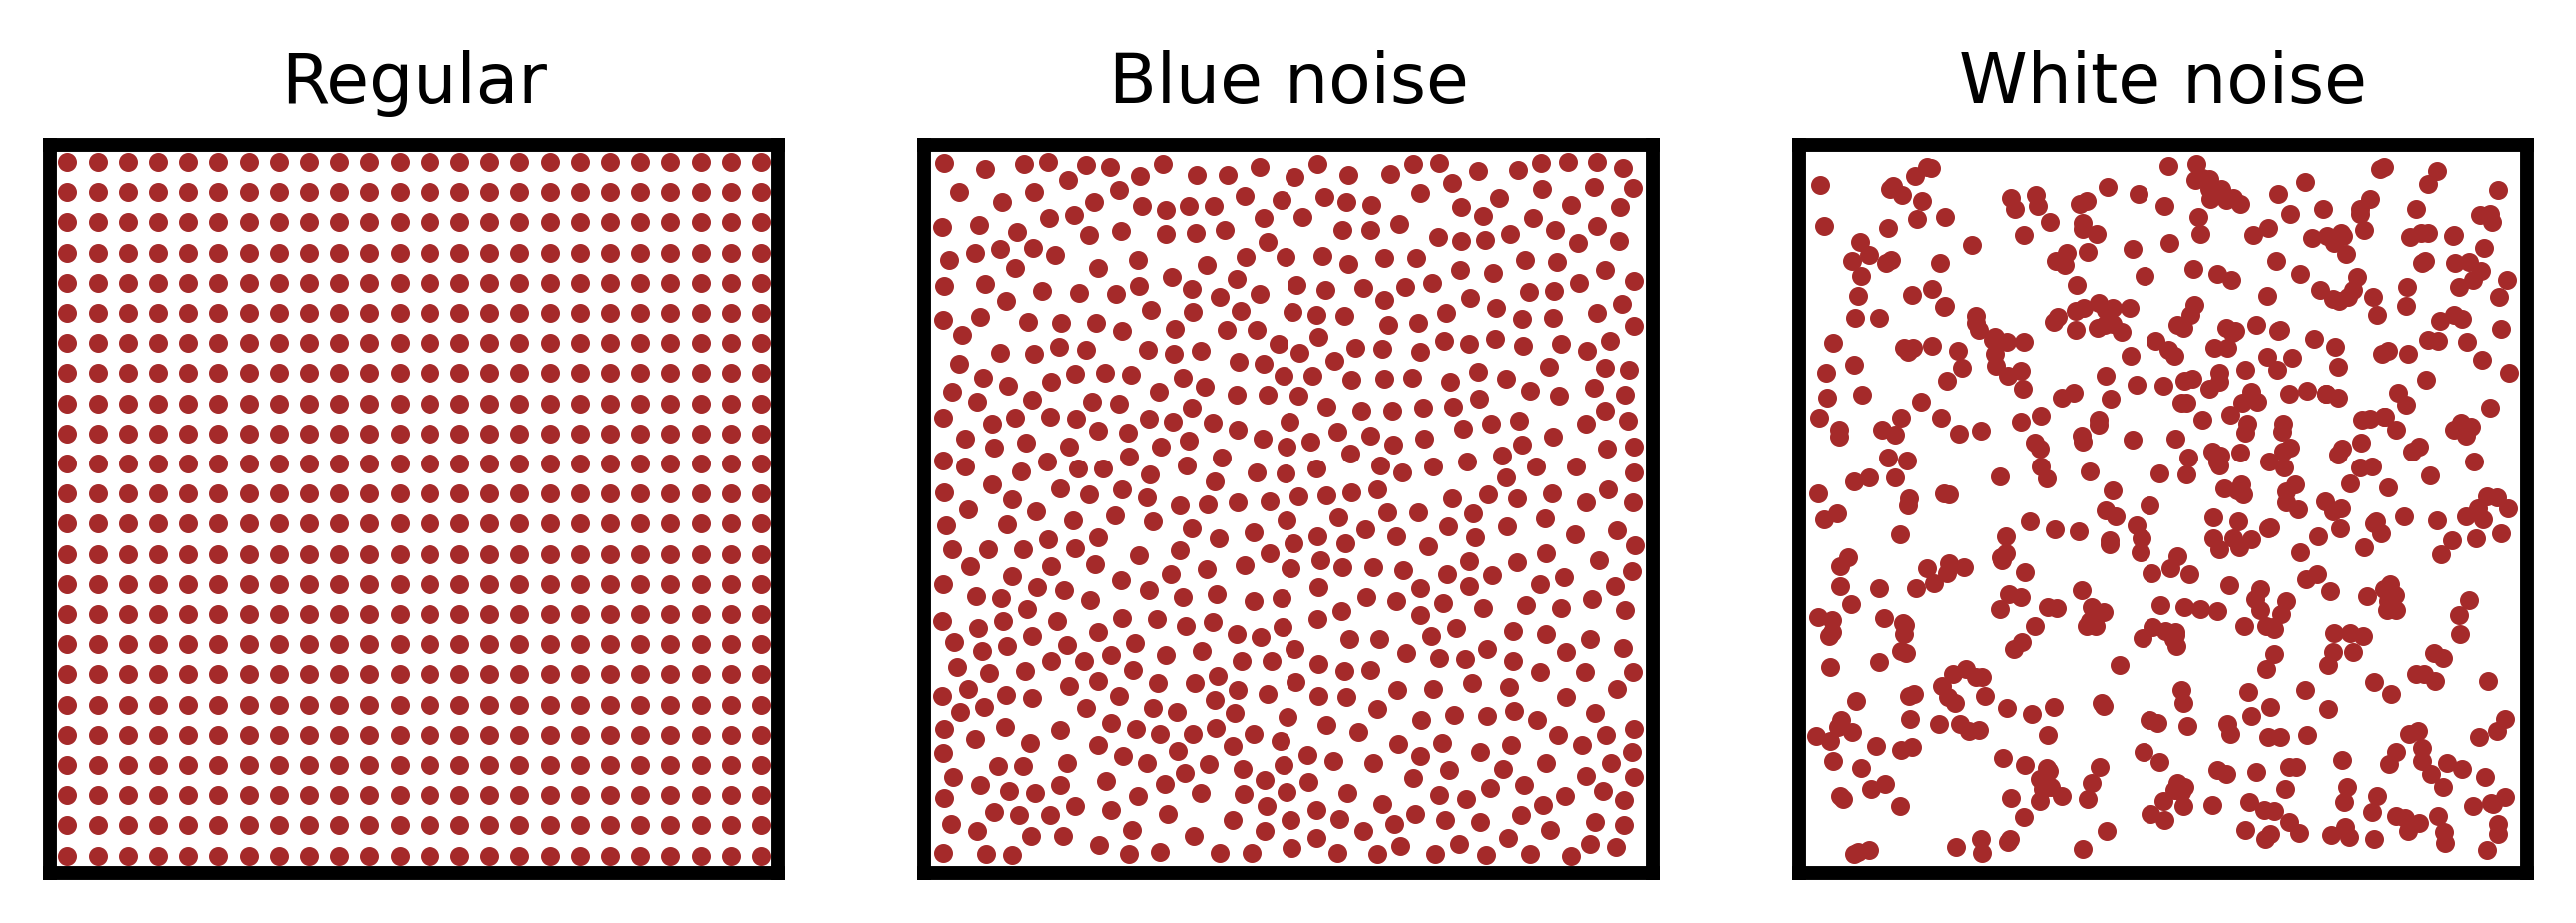
\includegraphics[width=15cm]{distribution_plot.png}
        \caption{Examples of the three kinds of input distributions. Each plot shows 24x24 inputs. Regular distribution places inputs evenly across the entire environment in a rectangular way. A blue noise distribution places inputs sequentially so each is placed as far away from other inputs as possible, resulting in an even, unstructured distribution. White noise distribution places inputs randomly, and independent of all other inputs, so some locations produce more input activity than others.}
        \label{distribution_plot}
    \end{figure}

    \subsection{Multi-Compartment Methods}
    One goal of this work was to investigate the nature of spatial inputs. While the section above describes how transition cells can obtain hexagonal activity with place-like inputs, previous work assumed that this input was conveyed to the transition cell through active computation in a dendritic tree. The spatial inputs given to this dendritic tree could have some other form, such as boundary vectors. To test the plausibility of this claim, this work made a network receiving direct spatial location, but instead of synapsing directly on the transition cell, it was transmitted through a non-spiking layer of dendrites. Dendritic activity would impact transition cells in ways like a gap-junction, modeling a continuously moving depolarization from the former to the latter. Nonlinear dendritic computation, in which the voltage of the dendrite was modulated both by a softmax function, and then a learned conductance, before impacting transition cell voltage, gave results comparable to the other models [figure 3.1, 3.6, see supplementary methods for a not-working model]. This indicates that dendrites can be used as units of active computation, but it depends heavily on the nonlinear dynamics of the dendrite.

    Notably, this multi-compartment model increases the computational load significantly, so this method was only attempted with the first set of parameters that gave decent results. This also impacts the upcoming section using BVCs as inputs.


    \section{Discussion}

    \subsection{Comparison to existing grid cell models}

    This work provides a network structure and learning rule that produces a cell-layer with grid-like activity from associating and dissociating to spatial inputs. Numerous other works has done this, each with their own set of assumptions. The benefit of feed-forward learning networks, compared to the popular CAN or OI -models, is that these models rely on external spatial information, and not self-velocity signals which can be prone to drift. That being said, there is rich support for CAN- and OI-models, and it is worth noting that these models are not directly antagonistic, instead seeking to explain different experimental grid cell observations.
    The major underlying assumption of this work, linking the observed grid cells to the theoretical transition cells of the TSS-model, is that grid cells receive spatial information in phase coded waves each theta cycle. From the perspective of TSS, phase coding the spatial relevance gives transition cell information about center- vs surround. Biologically, the utility of phase coding the input activity is that it naturally orients with spike timing dependent plasticity as a biologically plausible learning rule. At least two criteria are necessary for biological plausibility; first, that all learning relies on spatially locally available information, and secondly, that learning only uses information that is available at the time of learning [source]. While STDP has been observed experimentally [source?], having baseline modulation of weights depends only on input-information.  Compared to other models, the network does not rely on spike frequency adaptation [vs Kropff and Treves, for instance], and it does not rely on implausible learning rules such as backpropagation through time (BPTT) [source].

    However, despite the reasonably good gridness observed in this network structure, the within-simulation variance is quite high, with virtually all simulations containing some cells with negative scores. This was also seen in another simulation combining inhibition and excitation [Weber and Sprekeler]. Although all cells showed clearly isolated firing fields, both asymmetry and rectangular firing fields will produce negative gridness. It does seem like the local minimum state for most cells is a hexagonal firing pattern, but that other configurations that give zero or negative scores are moderately likely with this learning rule, possibly even necessary in a network. Additionally, from the temporal stability of the firing fields, there is indication that the cells with negative scores will be known early in the simulation, and only persist in their negative scores (can data support this?).


    \subsection{Comparison with existing TSS simulations}

    Transition cells, under the TSS-model, learn spatial transitions by associating to spatial information related to center-regions they encode transitions from, and dissociating from spatial information related to surround-regions, which they encode transitions to. A mechanism to support this is dense sampling, in which, in any given position, both spatial information from the places corresponding to center and the surround will be available [source: TSS thesis?]. This lets the transition cell acquaint to all spatial information, which is necessary to subsequently represent spatial transitions. Transition neurons also communicate laterally with inhibition, to discourage overlapping fields and representing the same transitions. 
    Prior to this work, all simulations of spatial learning under the TSS-model had unresolved questions that needed to be answered to be applicable in a biological network: how could a high number of transition neurons coexist in the network, and what would a biologically plausible learning rule look like? In the original simulations, inhibition times were instant, rate of learning was modulated by the number of inputs to account for edge effects, and the only input structure tested was one with a rectangular distribution.
    Compared to this, this work is a decisive step in the direction of biological plausibility, showing high degrees of gridness in larger networks, as well as uniform phase distributions. Although this work did not show explicit hexagonality with BVC-inputs, it showed gridness with different input distributions, a smaller number of dendrites (576 vs 2304) and only velocity-based learning rate modulation.

    Existing simulations of the TSS model had a third learning rule, an interaction rule, in which transition cells dissociated from spatial information whenever another transition cell activated first. This learning rule wasn't implemented here because it wasn't clear how - one plausible alternative is that receiving inhibition would decrease weights, but this was technically difficult to implement with the simulation library used, and would have increased simulation times. However, a learning rule like this might encourage faster convergence and a wall-angle orientation closer to the 7.5 degrees that might be expected, due to its high number of packed center-surround areas. On the other hand, this learning rule might also strain the network more in terms of size, because it discourages overlapping fields.

    \subsection{The future: benefits of BVCs, biological plausibilities etc}

    Considering that optic flow can explain boundary vector cell activity from pure visual inputs, a network producing gridlike cells from BVC-inputs is desirable because it explains how spatial transitions can be learnt from sensory information available at the time of exploration. Under certain conditions, it might also extrapolate to other vector-based inputs, such as object-vector cells, given that these cells can also be modeled from optic flow, and that there is a sufficient number of landmarks to triangulate positional information from. Although this work by no means is conclusive on the nature of such a network, nor any concrete data on the BVC-to-transition cell network, it provides some predictions at what such a network should look like.

    Importantly, because most BVCs will be active in both the center- and the surround-region of the transition cell [supplementary models, I guess], linear summation of all boundary vector cell activity is unlikely to yield effective transition cells. Instead, some nonlinear process is necessary to allow transition cells to respond to BVCs in some locations, and not in others. In this work, the mechanism that supports this is dendritic computations, in which each dendrite receives a subset of BVC-inputs, and the transition cell in practice can learn on each dendrite, instead of individual inputs. This idea followed both experimental data on superlinear activation of pyramidal grid cell dendrites [source], as well as a model using dendritic computations to explain place cell remapping [source]. In this model, each dendrite adapted to some place in some environment, and context-signals would inhibit all dendrites except the one governing the current environment. This allowed the place cell to remap orthogonally.

    Using the same idea in this work, so each dendrite would represent some location in the environment, the learning variable was the dendrite conductance, and not synaptic weights. This isn't grounded in experimental observations, but rather two reasons of model clarity: first, that this mimics models in which place-like spatial inputs synapse onto grid cells, such as the other models in this work. This clarifies comparison, because the learning variable always has the same functional role in the network, as place-input to grid-cell weights. Secondly, although not directly explored here, one way of self-organizing BVC- to dendrite-connectivity is by randomly connecting a superfluous number of BVCs on each dendrite, and pruning unnecessary connections so the dendrite activates in only one or a few places. Differentiating between these two kinds of learning - BVC-to-dendrite and dendrite-to-grid cell, was thought to make these processes easier to distinguish. 
    This model provides the testable hypothesis that 1) dendrites will exhibit place-like activity fields during traversing of familiar environments, and 2) only depolarization in dendrites which represent places that are within the hexagonal grid pattern will contribute to somatic depolarization and grid cell spiking. 

    That being said, there is no central limitation that learning has to occur in dendrite-to-grid cell conductances. Alternatively, the STDP-learning signal must be transmitted to all postsynapses in the dendrite, in which all the weights will be changed indiscriminately, except possibly those pruned in mechanisms described in the above paragraph. In this case, it is also possible that all dendrites end up with place fields within the grid pattern.

    One of the most direct predictions from this work is that in the case of such a dendritic input tree, the distribution of place-like inputs to the grid cell should be relatively evenly distributed spatially. With LIF model neurons, it seems more difficult to converge on proper gridness when inputs have place fields that are uniformly and independently distributed. A more even distribution, such as a blue noise pattern, is for instance seen in the layout of cones in the human retina, but to make dendrites activate in a blue noise pattern would require some mechanism, for instance by making them disassociate from each other.

    Some further challenges underlie the model relying on an expansive dendritic tree as a hidden layer between vectorized inputs and grid-like transition cells. Not only is the number of dendrites required too high compared to that of both stellate and pyramidal principal mECII cells, but if each dendrite should correspond to one location, the required number of dendrites required would need to scale linearly with the number of places visited. If inspiration is again taken from what is known of hippocampal place cells, some kind of context modulation or remapping might help explain this, but significant work is required to highlight how this would work. With BVC-input, the same dendrite would in principle respond to the same place in multiple environments, as long as the boundary information is similar, so each dendrite could be reused across contexts as long as conductances could be modulated across environments. Prior to exploring this in the engineer-like simulations like this work has done, this question should be investigated in a theoretical framework.
    It is, however, in the spirit of the TSS to assume that the dendrites of a transition cell serves some computational purpose, and does this well.




    \printbibliography

\end{document}